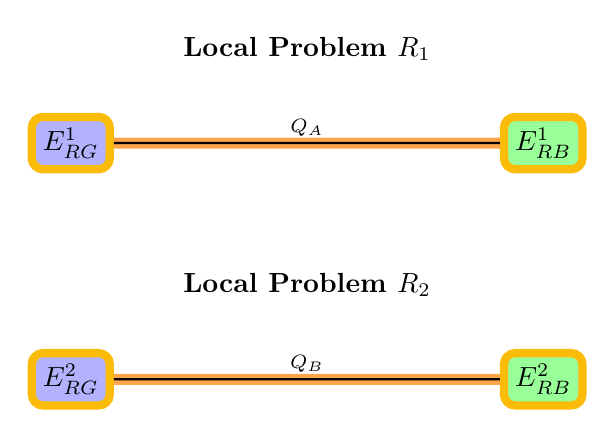
\begin{tikzpicture}[scale=1.5,
    nodeRG/.style={rectangle, rounded corners, draw=black, thick, fill=blue!30, inner sep=4pt, minimum width=24pt, minimum height=16pt},
    nodeRB/.style={rectangle, rounded corners, draw=black, thick, fill=green!40, inner sep=4pt, minimum width=24pt, minimum height=16pt},
    active/.style={draw=yellow!50!orange, line width=3pt}]

    % Group for R1
    \node[nodeRG, active] (RG1) at (-2, 1) {$E_{RG}^1$};
    \node[nodeRB, active] (RB1) at (2, 1) {$E_{RB}^1$};
    
    % Group for R2
    \node[nodeRG, active] (RG2) at (-2, -1) {$E_{RG}^2$};
    \node[nodeRB, active] (RB2) at (2, -1) {$E_{RB}^2$};

    % Physical qubits (Only ones sharing the same Red vertex)
    \draw[black!20, thick] (RG1) -- (RB1);
    \draw[black!20, thick] (RG2) -- (RB2);

    % Selected paths by MWPM (disjoint!)
    \draw[orange, line width=4pt, opacity=0.7] (RG1) -- (RB1);
    \draw[orange, line width=4pt, opacity=0.7] (RG2) -- (RB2);
    
    \draw[black, thick] (RG1) -- (RB1) node[midway, above, sloped, font=\scriptsize, text=black, inner sep=2pt] {\textbf{$Q_A$}};
    \draw[black, thick] (RG2) -- (RB2) node[midway, above, sloped, font=\scriptsize, text=black, inner sep=2pt] {\textbf{$Q_B$}};
    
    \node at (0, 1.8) {\textbf{Local Problem $R_1$}};
    \node at (0, -0.2) {\textbf{Local Problem $R_2$}};
    
\end{tikzpicture}